\subsection{Arquitectura global}

\begin{figure}[H]
\centerline{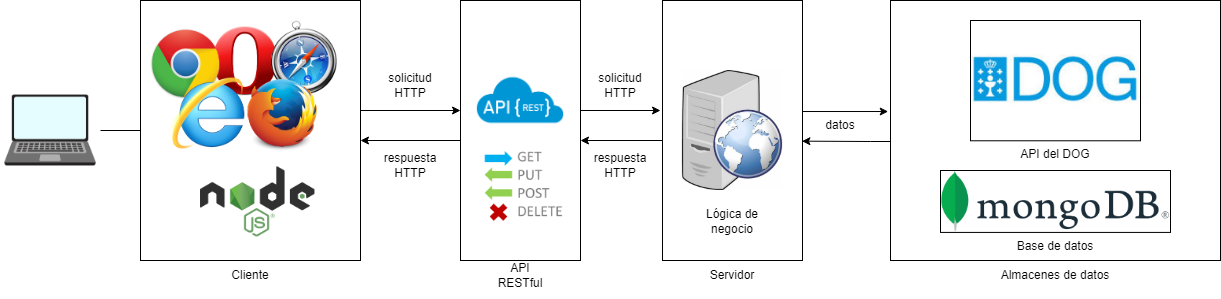
\includegraphics[width=15cm]{figuras/diseño/arquitecturaglobal.PNG}}
\caption{Arquitectura global del sistema.}
\label{enlaceArquitecturaGlobal}
\end{figure}

En la arquitectura global del sistema se pueden diferenciar tres componentes: el cliente, el servidor y los almacenes de datos.
\\

El cliente está conformado por todos aquellos navegadores web que realizan llamadas a la API del servidor mediante su propia interfaz. Todo esto se ha realizado gracias a Node.js \cite{nodejs}, el entorno de ejecución de JavaScript del proyecto.
\\

De todas formas, existen algunos clientes web, como por ejemplo Internet Explorer \cite{explorer}, los cuales han quedado obsoletos. En el caso de estos navegadores, no las tecnologías no tienen soporte y la aplicación no funcionará correctamente.
\\

Desde el cliente se realizan solicitudes HTTP hacia el servidor, que expone todos sus servicios en una API. Con ello, el cliente intercambia información con el servidor según la llamada realizada: GET para obtener información, POST para crear objetos, PUT y PATCH para modificar información, y DELETE para eliminar objetos.
\\

La información que el servidor obtiene ha de recuperarla y almacenarla en algún sitio. En el caso de la API del DOG, solo recibe información de esta, obteniendo las leyes almacenadas en el servidor del DOG. Con respecto a la base de datos de MongoDB \cite{mongodb}, de esta puede obtener información, almacenar datos, modificar y eliminar.
\\

En cuanto a la base de datos empleada (MongoDB), cabe mencionar que esta es una base de datos NoSQL \cite{nosql}. Este tipo de bases de datos se caracterizan por orientadas hacia documentos, y almacenan y recuperan los datos en formatos que no son tablas.
\\

Con esta arquitectura se ha logrado el cumplimiento de dos requisitos no funcionales descritos: el {\bf NFR-08: Uso de tecnologías web y servicios RESTful} (uso de Node.js) y el {\bf NFR-09: Base de datos NoSQL}.